\documentclass[10pt]{article}

\usepackage[utf8]{inputenc}
\usepackage{floatrow}

\usepackage{algorithm}
\usepackage{algorithmic}
\usepackage[T1]{fontenc}
\usepackage{enumitem}
\usepackage{hyperref}
\usepackage{graphicx}
\usepackage{color}
\usepackage{listings}
\usepackage{wrapfig}
\usepackage{amsfonts}
\usepackage{amsmath}
\usepackage{mathtools}
\usepackage[hmargin=1.25in,vmargin=1.25in]{geometry}
\newcommand{\shellcmd}[1]{\\\indent\indent\texttt{\footnotesize\# #1}\\}
  
%title setup
\title{Projet informatique: Honshu (Lot B)}
\author{
  Romain PEREIRA\\
  Douha OURIMI\\
  Afizullah RAHMANY\\
  Guangyue CHEN
}
\date{08/04/2018}

% table of contents setup
\renewcommand{\contentsname}{Sommaire}
\usepackage{etoolbox}
\patchcmd{\thebibliography}{\section*{\refname}}{}{}{}

\hypersetup{
  colorlinks,
  citecolor=black,
  filecolor=black,
  linkcolor=blue,
  urlcolor=red
}

\begin{document}
  \maketitle
  \tableofcontents
  
  \newpage
  \section*{Préambule}
  Ce projet est réalisé dans le cadre de nos études à l'ENSIIE.
  L'objectif est de prendre en main des outils de 'programmation agile',
  en developpant un jeu de carte : le Honshu.
  \newline
  \begin{figure}[H]
    \begin{center}
      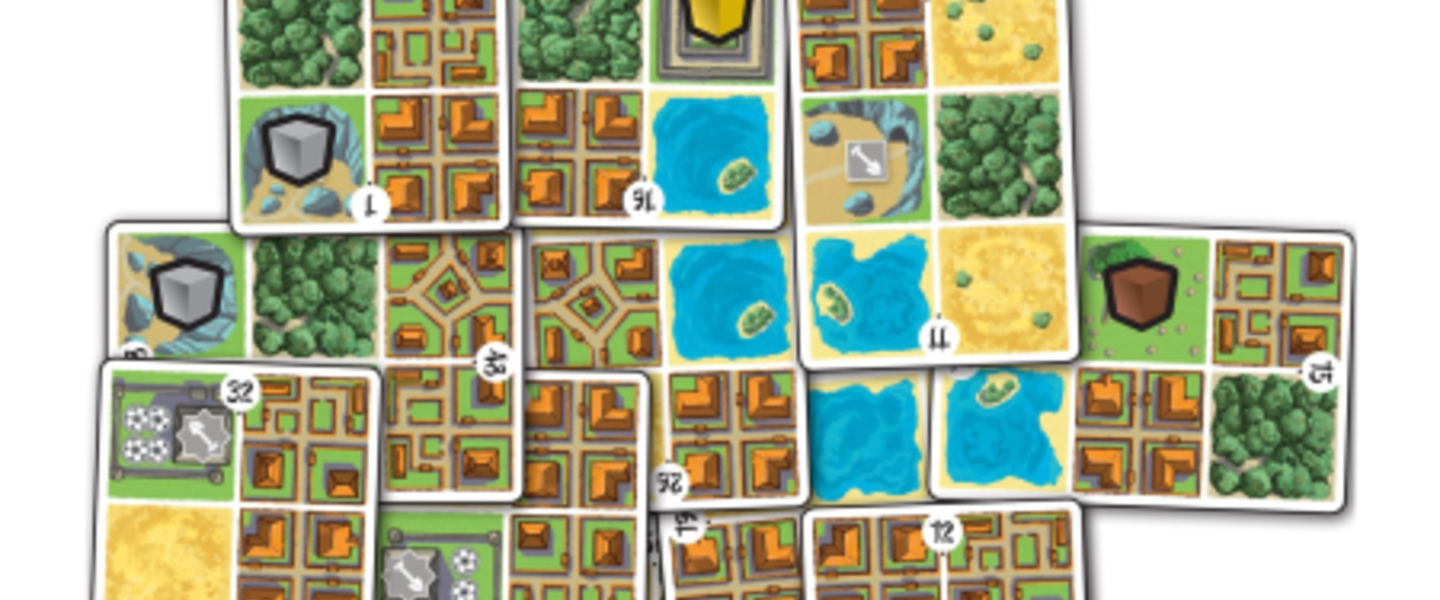
\includegraphics[height=6cm,keepaspectratio]{../images/honshu.png}
    \end{center}
    \caption{\textit{Plateau de jeu}}
    \label{honshu_introduction}
  \end{figure}
  
  \section{Introduction}
    Nous voici dans la deuxième partie du projet. Pour ce lot nous étions en charge de la réalisation d'un jeu avec affichage en mode terminale. Comme une partie du lot B a déjà été réalisée lors du lot précèdant nous avons décidé de scinder le groupe en deux parties et de faire deux affichages différents. 
    L'un répondant stricto sensu au demande du lot B et un autre visuellement plus agréable et user-friendly.
    Le travail a été donc réparti de la manière suivante :
    \newline
      - Guangyue et Romain ont été en charge d'un affichage avec la bibliothèque ncurses en mode terminale.
      Cette bibliothèque permet un rendu visuellement plus esthétique de manière plus aisée.
      \newline
      - Douha et Afizullah ont été en charge d'un affichage avec en mode terminale avec toutes les fonctions écrites ex nihilo :
	\begin{itemize}[label=-]
	  \item Afizullah a implémenté l'affichage de la gille et des cartes en main.
	  \item Douha était en charge des entrées. Il s'agit d'implémenter l'interaction qu'aura le joueur avec l'état du jeu.
	\end{itemize}
    Les deux modes de rendu sont accessibles en recompilant le jeu avec les commandes:
    \newline
    \shellcmd{make MODE=ncurses} ou \shellcmd{make MODE=standart}\newline
    Nous étions également en charge des tests de recouvrement et de la limitation de la zone de jeu. 
    Il convient de préciser que les tests de recouvrement ont été réalisés de manière intrinsèque lors de l'implémentation du lot précèdant
  \newpage
  \section{Rapport lot B}
  \subsection{Interfaces 'affichage.h' et 'entree.h'}
      Ces interfaces définissent les structure et les fonctions devant être implémentées pour un type d'affichage ou de rendu.
      Les 2 modes (standard et ncurses) ont chacun une implémentation différente ('src/standart/', et 'src/ncurses'),
      mais tout le reste du code reste inchangé: le Makefile s'occupe de compiler avec la bonne implémentation.
      
  \subsection{1ère implémentation}
  \subsubsection{Partie affichage}
        \paragraph{affichage.h}
      Il s'agit d'afficher la grille, et les tuiles dans la main du joueur. 
      En effet, chaque case de la grille possède un attribut type qu'il convient
      de convertir en un caractère (à l'aide la fonction case\_char) qu'on affichera ensuite dans
      l'emplacement ad hoc dans la grille affichée.
      La connaissance des tuiles sur la grille n'est pas nécessaire, en revanche, c'est le cas pour l'affichage
      de la main du joueur. Pour discriminer une tuile dans la main et une tuile posée sur la grille, 
      on se sert du flag présent de la structure tuile indiquant si celle-ci est sur la grille ou non.
      \begin{center}
	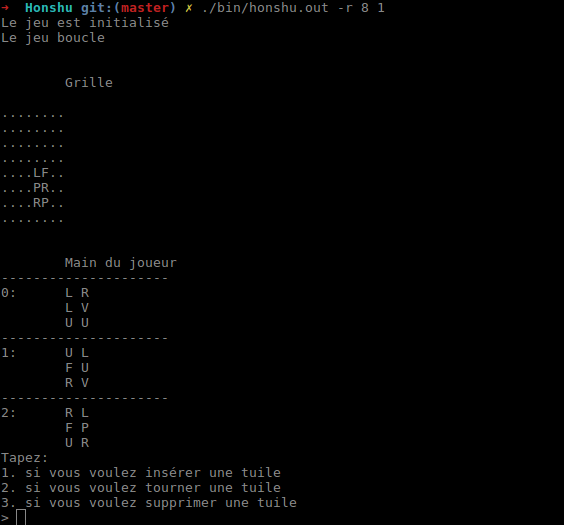
\includegraphics[height=6cm,keepaspectratio]{../images/grille_standart.png}
      \end{center}
      
  \subsubsection{Partie entrée}
       \paragraph{entree.h}
      Il s'agit d'implémenter la manière dont le joueur pourra interagir avec la partie. L'input du joueur sera interprété pour que celle-ci modifie
      la grille et les tuiles de la partie donc les structure ad hoc.
      On offre au joueur la possibilité d'insérer, faire pivoter ou supprimer une tuile. Ces possibilités sont offertes par les fonctions
      $grille\_insert$ et $grille_can_insert$
      qui assure les tests de recouvrement et de limitation de la grille.
      En effet une tuile est décrite par son orientation et par sa coordonnée qui correspond à celle de sa case en haut à gauche.
      On vérifie qu'elle ne recouvre ni une case ni entièrement une autre tuile ni ne dépasse de la grille et recouvre au moins une case.
      Une tuile ne peut être insérée à travers la fonction $grille\_insert$ que si elle a été passée en argument de la fonction $grille\_can\_insert$
      et a retourné 1.  On peut alors  rafraîchir l'affichage à travers la boucle de jeu.
  \subsection{2ème implémentation avec ncurses}
  \paragraph{Affiche le jeu:} Celle-ci étant plus technique, elle a été décrite par les algorithmes suivants.
  \subsubsection{Partie affichage}
  
  \paragraph{Affiche le jeu:} 
  Affiche la grille, les tuiles dans la main ainsi la tuile sélectionnée et présentement sur la grille.
  Les tuiles ayant des états différents auront des couleurs différentes
  (celle qui est séléctionnée sera soit vert si l'insertion est possible, rouge sinon..
  
  \begin{algorithm}
    \caption{Affiche le jeu}
    \begin{algorithmic}
      \STATE Affiche le titre
      \STATE Affiche les tuiles
      \STATE Affiche la grille
      \STATE Affiche la tuile selectionnée dans la grille
      \STATE Affiche les commandes de jeu.
    \end{algorithmic}
  \end{algorithm}	
  \paragraph{Affiche toutes les tuiles}
  Affiche les tuiles dans des couleurs différentes suivant leur état et si elles sont séléctionnées par le joueur.
  \begin{algorithm}
    \caption{Affiche toutes les tuiles}
    \begin{algorithmic}
      \REQUIRE  une structure de \textit{honshu} ;
      \ENSURE renvoie Void, et affiche les tuile dans le terminal
      \STATE affiche le titre
      \STATE \textit{x} $\leftarrow$ \textit{Index\_de\_tuile}$\% 2 * 7$
      \STATE \textit{y} $\leftarrow$ \textit{Index\_de\_tuile}$/ 2 * 7$
      \FOR{Chaque \textit{tuile} de \textit{Honshu}}
      \STATE \textit{tuile\_à\_affiche} $\leftarrow$ \textit{Honshu}.tuile
      \IF{\textit{tuile\_à\_affiche} est SUR\_CARTE}
      \STATE change la couleur en rouge
      \ENDIF
      \STATE Rappelle la fonction \textit{afficher\_une\_tuile} et affiche \textit{tuile\_à\_afficher} en (x,y)
      \ENDFOR
    \end{algorithmic}
  \end{algorithm}
  \paragraph{Affiche une tuile:}
  Affiche une tuile dans le terminale, si elle est déjà selectionnée, sa couleur change.
  \begin{algorithm}
    \caption{Affiche une tuile}
    \begin{algorithmic}
      \REQUIRE  une \textit{tuile} et deux coordonnées (\textit{x} , \textit{y} ) ; 
      \ENSURE Renvoie Void, et affiche une tuile en (\textit{x},\textit{y})
      \FOR{Chaque \textit{case} de \textit{tuile}}
      \STATE Par la \textit{rotation} de la \textit{tuile}, déduire la place de ces \textit{cases}
      \STATE Rappelle la fonction \textit{case\_char} et affiche le caractère correspondant au type de la case
      \ENDFOR
    \end{algorithmic}
  \end{algorithm}						
  \paragraph{Affiche le grille:}Affiche la grille dans le terminale.
    \begin{algorithm}
      \caption{Affiche la grille}
      \begin{algorithmic}
	\REQUIRE  une structure de \textit{honshu} ;
	\ENSURE renvoie Void, et affiche la grille dans le terminale
	\STATE \textit{grille} $\leftarrow$ \textit{Honshu}.grille
	\STATE affiche le titre
	\FOR{Chaque \textit{case} de la\textit{grille}}
	\STATE \textit{cases} $\leftarrow$ \textit{grille}.case (par rappel de la fonction \textit{grille\_get})
	\IF{\textit{case} != NULL }
	\IF{\textit{case} est dans une tuile affichée }
	\STATE la tuile prend la couleur rouge
	\ENDIF
	\ENDIF
	\STATE Affiche les \textit{cases}
	\ENDFOR
      \end{algorithmic}
    \end{algorithm}
    \begin{center}
      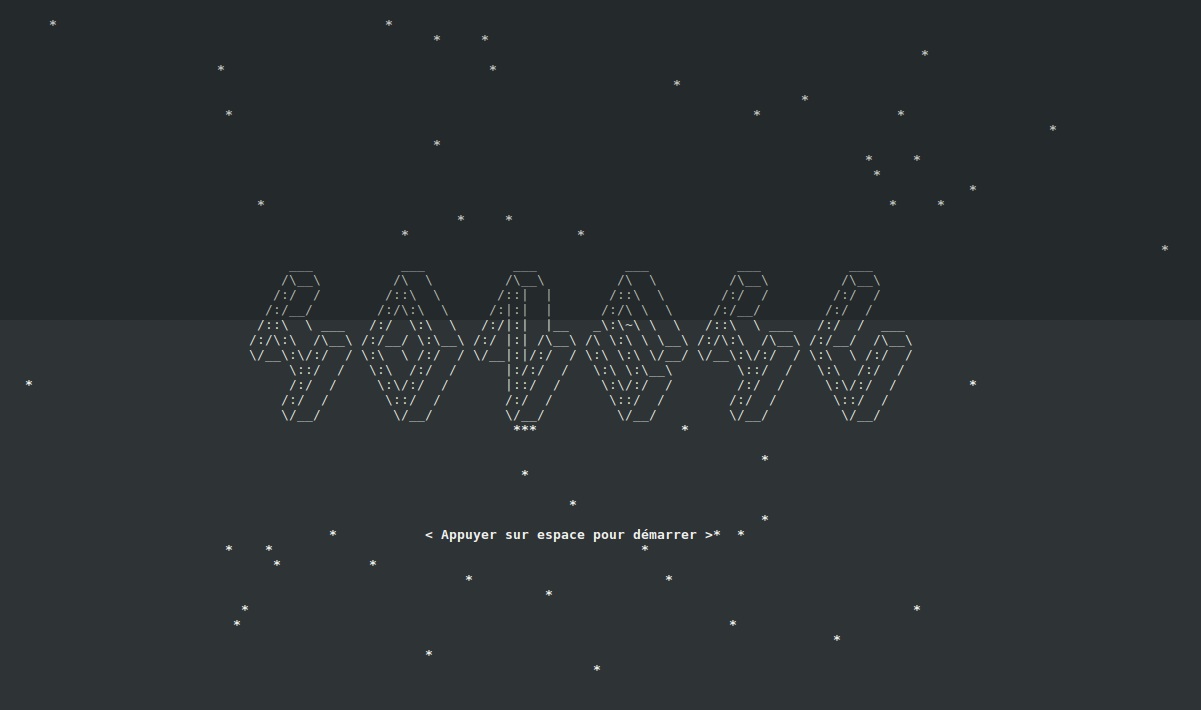
\includegraphics[height=6cm,keepaspectratio]{../images/menu_ncurses.png}
    \end{center}
    \begin{center}
      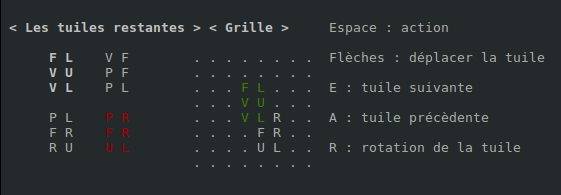
\includegraphics[height=6cm,keepaspectratio]{../images/grille_ncurses.png}
    \end{center}
  \subsubsection{Partie entrée}
    L'implémentation avec 'ncurses' a été rapide, grâce au travail effectué au lot A. Ncurses fourni une fonction $$getch()$$ qui lit un caractère sur l'entrée standard. Une action a été attribuée à chaque touche,
    voir $ncurses/entree.c$ pour plus de détails.
  \section{Conclusion}
    Pour ce lot, nous avons mis en place un système d'entrée/sortie modulaire, qui nous a permis de tous travailler en parallèle efficacement.
    Grâce à cette séparation du travail efficace, nous n'avons eu que peu (voir pas) de 'fusion' (merge) de code à effectuer.
    De plus, ce système d'interface entrée/sortie nous a permis d'implémenter rapidement 2 interfaces graphiques différentes,
    et pourra être amplement ré-utilisée pour le lot D (affichage avec SDL). Pour la suite nous préférons garder l'implémentation avec ncurses car elle est plus performante et aboutie. 
    Il nous restera à réfléchir à l'implémentation du solveur sachant que l'algorithme proposé (testant toutes les possibilités d'insertion)
    a été imaginé lors du choix des structures pendant le lot A.

  
\end{document}
